\documentclass{article}

\usepackage[T1]{fontenc}
\usepackage[utf8]{inputenc}
\usepackage[french]{babel}
\usepackage{graphicx}
\usepackage{float}
\usepackage{longtable}
\usepackage{booktabs}
\usepackage{listings}
\usepackage{xcolor}
\usepackage{hyperref}

\lstset{
  basicstyle=\ttfamily\footnotesize,
  breaklines=true,
  breakatwhitespace=true,
  columns=fullflexible,
  keepspaces=true,
  frame=single,
  numbers=left,
  numberstyle=\tiny,
  captionpos=b,
  showstringspaces=false
}

\title{Analyse des thèmes dans les romans de Zola}
\author{Morgan RICHARD}
\date{}

\begin{document}

\maketitle

\section{Introduction}

Émile Zola, l'un des écrivains les plus célèbres du XIXe siècle, est connu pour ses romans naturalistes qui explorent les aspects sociaux, économiques et psychologiques de la vie humaine. 

Dans cette analyse, nous allons examiner les thèmes récurrents dans les œuvres de Zola et déterminer s'ils apparaissent dans plusieurs de ses romans. Des méthodes d'analyse textuelle seront utilisées pour identifier les thèmes principaux à travers les différents romans.

La question centrale de cette étude est donc la suivante : dans quelle mesure des méthodes non supervisées comme le NMF et K-means permettent-elles de faire apparaître des structures thématiques récurrentes dans l'œuvre romanesque de Zola ?

L'objectif est de vérifier si les regroupements produits automatiquement correspondent à des motifs interprétables dans le cadre d'une analyse littéraire.

Ce travail est le premier d'une série d'analyses portant sur un corpus de textes littéraires issus de différents auteurs naturalistes et non naturalistes.

Deux méthodes d'analyse ont été utilisées pour identifier les thèmes dans les romans de Zola : 
\vspace{0.5cm}
\begin{itemize}
\item le NMF (Non-negative Matrix Factorization)\footnote{N. Gillis, \textit{Nonnegative Matrix Factorization}, Society for Industrial and Applied Mathematics, coll. « Data Science », 2020.} : une technique de réduction de dimensionnalité qui permet d'extraire des thèmes à partir d'un corpus de textes. 

\item K-means : une méthode de clustering qui permet de regrouper les thèmes récurrents en fonction de leur similarité thématique.
\end{itemize}
\vspace{0.5cm}
Ces méthodes seront expliquées en détail dans les sections suivantes, où nous présenterons les résultats de l'analyse thématique des romans de Zola.


\section{Présentation du corpus}

Comme indiqué en introduction, cette étude porte sur un corpus composé exclusivement de romans d'Émile Zola. Le choix a été fait de ne pas inclure les nouvelles, les textes journalistiques ni les essais, afin de conserver un ensemble relativement homogène du point de vue générique. Les romans offrent en effet une matière textuelle plus longue et plus développée, ce qui permet d'observer plus finement les thèmes récurrents, les milieux sociaux et les motifs narratifs présents dans l'œuvre de Zola.

L'exclusion des nouvelles répond également à une contrainte méthodologique. Ces textes sont généralement plus courts que les romans et leur intégration aurait pu créer un déséquilibre dans le corpus. Dans le cadre d'une analyse thématique fondée sur des segments textuels, les différences importantes de longueur entre les œuvres peuvent influencer la représentation des thèmes. Limiter le corpus aux romans permet donc de réduire cet effet et de travailler sur un ensemble plus comparable.

Le corpus comprend les œuvres suivantes :

\begin{longtable}{p{1.6cm}p{4.2cm}p{8cm}}
\caption{Corpus des œuvres de Zola utilisées dans l'analyse}\\
\toprule
\textbf{Date} & \textbf{Titre} & \textbf{Fichier} \\
\midrule
\endfirsthead

\toprule
\textbf{Date} & \textbf{Titre} & \textbf{Fichier} \\
\midrule
\endhead

1865 & \textit{La confession de Claude} & \texttt{1865\_La\_confession\_de\_Claude.\_clean.txt} \\
1866 & \textit{Le vœu d'une morte} & \texttt{1866\_Le\_voeu\_d\_une\_morte.\_clean.txt} \\
1867 & \textit{Les mystères de Marseille} & \texttt{1867\_Les\_mysteres\_de\_Marseille.\_clean.txt} \\
1867 & \textit{Thérèse Raquin} & \texttt{1867\_Therese\_Raquin.\_clean.txt} \\
1868 & \textit{Madeleine Férat} & \texttt{1868\_Madeleine\_Ferat.\_clean.txt} \\
1871 & \textit{La fortune des Rougon} & \texttt{1871\_1\_La\_fortune\_des\_Rougon.\_clean.txt} \\
1872 & \textit{La curée} & \texttt{1871\_2\_La\_curee.\_clean.txt} \\
1873 & \textit{Le ventre de Paris} & \texttt{1873\_3\_Le\_ventre\_de\_Paris.\_clean.txt} \\
1874 & \textit{La conquête de Plassans} & \texttt{1874\_4\_La\_conquete\_de\_Plassans.\_clean.txt} \\
1875 & \textit{La faute de l'abbé Mouret} & \texttt{1875\_5\_La\_faute\_de\_l\_abbe\_Mouret.\_clean.txt} \\
1876 & \textit{Son Excellence Eugène Rougon} & \texttt{1876\_6\_Son\_Excellence\_Eugene\_Rougon.\_clean.txt} \\
1877 & \textit{L'assommoir} & \texttt{1877\_7\_L\_assommoir.\_clean.txt} \\
1878 & \textit{Une page d'amour} & \texttt{1878\_8\_Une\_page\_d\_amour.\_clean.txt} \\
1880 & \textit{Nana} & \texttt{1880\_9\_Nana.\_clean.txt} \\
1882 & \textit{Pot-Bouille} & \texttt{1882\_10\_Pot-bouille.\_clean.txt} \\
1883 & \textit{Au Bonheur des dames} & \texttt{1883\_11\_Au\_Bonheur\_des\_dames.\_clean.txt} \\
1884 & \textit{La joie de vivre} & \texttt{1884\_12\_La\_joie\_de\_vivre.\_clean.txt} \\
1885 & \textit{Germinal} & \texttt{1885\_13\_Germinal.\_clean.txt} \\
1886 & \textit{L'œuvre} & \texttt{1886\_14\_L\_oeuvre.\_clean.txt} \\
1887 & \textit{La terre} & \texttt{1887\_15\_La\_terre.\_clean.txt} \\
1888 & \textit{Le rêve} & \texttt{1888\_16\_Le\_reve.\_clean.txt} \\
1890 & \textit{La bête humaine} & \texttt{1890\_17\_La\_bete\_humaine.\_clean.txt} \\
1891 & \textit{L'argent} & \texttt{1891\_18\_L\_argent.\_clean.txt} \\
1892 & \textit{La débâcle} & \texttt{1892\_19\_La\_debacle.\_clean.txt} \\
1893 & \textit{Le docteur Pascal} & \texttt{1893\_20\_Le\_docteur\_Pascal.\_clean.txt} \\
1894 & \textit{Lourdes} & \texttt{1894\_1\_Lourdes.\_clean.txt} \\
1896 & \textit{Rome} & \texttt{1896\_2\_Rome.\_clean.txt} \\
1898 & \textit{Paris} & \texttt{1898\_3\_Paris.\_clean.txt} \\
1899 & \textit{Fécondité} & \texttt{1899\_1\_Fecondite.\_clean.txt} \\
1901 & \textit{Travail} & \texttt{1901\_2\_Travail.\_clean.txt} \\
1903 & \textit{Vérité} & \texttt{1903\_3\_Verite.\_clean.txt} \\

\bottomrule
\end{longtable}

Le corpus est composé de 31 romans, qui couvrent les principales périodes de la production romanesque de Zola. Il comprend :

\begin{itemize}
    \item 5 romans antérieurs au cycle des \textit{Rougon-Macquart} ;
    \item 20 romans appartenant au cycle des \textit{Rougon-Macquart} ;
    \item 3 romans du cycle des \textit{Trois Villes} ;
    \item 3 romans publiés du cycle des \textit{Quatre Évangiles}.
\end{itemize}

Pour ce qui est des \textit{Quatre Évangiles}, \textit{Vérité} paraît à titre posthume. \textit{Justice} ne paraîtra jamais, l'ouvrage étant resté à l'état d'ébauche au moment de la mort de l'écrivain.

Ce corpus permet donc de couvrir une large période de la carrière de Zola, depuis ses premiers romans jusqu'à ses dernières œuvres. Cette amplitude chronologique est importante pour l'analyse, car elle permet d'observer non seulement les thèmes récurrents de l'œuvre romanesque, mais aussi leur possible évolution au fil du temps\footnote{En vue d'une éventuelle analyse ultérieure par dynamic topic modeling sur ce même corpus.}.
\section{Méthodologie de préparation des données}

Dans cette étude, le terme \textit{topic} désigne un regroupement lexical produit par le modèle NMF, tandis que le terme \textit{cluster} désigne un groupe de segments obtenu par K-means. Le terme \textit{thème} est réservé à l'interprétation qualitative de ces regroupements. Cette précision terminologique est importante pour éviter toute confusion entre les différentes étapes de l'analyse.

\subsection{Préparation des données brutes en données propres}

Les romans au format \texttt{.txt} correspondent à des versions nettoyées, c'est-à-dire à des textes dont les éléments non textuels ont été supprimés. Ces éléments comprennent notamment les titres, les chapitres, les notes de bas de page et d'autres informations éditoriales qui pourraient perturber l'analyse. Ce nettoyage permet d'obtenir une représentation plus précise des thèmes présents dans les romans.

De plus, le choix a été fait de conserver une seule phrase par ligne. Ce format facilite l'analyse textuelle, notamment pour les méthodes de la NMF et de K-means, qui nécessitent une structure de données homogène pour fonctionner correctement.

Cette logique de formatage a également été appliquée en prévision des analyses futures. Les romans issus de prochains traitements pourront ainsi être intégrés de manière cohérente au corpus. Ce choix permet de limiter les différences de structure entre les fichiers et d'obtenir un format homogène pour l'analyse sans trop complexifier le processus de préparation des données.

\begin{longtable}{p{8cm}r}
\caption{Nombre de tokens par roman dans l'ordre chronologique}  \\
\toprule
\textbf{Titre du roman} & \textbf{Nombre de tokens} \\
\midrule
\endfirsthead

\toprule
\textbf{Titre du roman} & \textbf{Nombre de tokens} \\
\midrule
\endhead

La confession de Claude & 47253 \\
Le vœu d'une morte & 38722 \\
Les mystères de Marseille & 125253 \\
Thérèse Raquin & 66363 \\
Madeleine Férat & 97318 \\
La fortune des Rougon & 116685 \\
La curée & 105120 \\
Le ventre de Paris & 110442 \\
La conquête de Plassans & 113245 \\
La faute de l'abbé Mouret & 114667 \\
Son Excellence Eugène Rougon & 126186 \\
L'assommoir & 158340 \\
Une page d'amour & 102185 \\
Nana & 141573 \\
Pot-Bouille & 134844 \\
Au Bonheur des dames & 147521 \\
La joie de vivre & 117255 \\
Germinal & 164473 \\
L'œuvre & 130613 \\
La terre & 163687 \\
Le rêve & 66379 \\
La bête humaine & 125418 \\
L'argent & 143010 \\
La débâcle & 187046 \\
Le docteur Pascal & 112713 \\
Lourdes & 173511 \\
Rome & 233958 \\
Paris & 177389 \\
Fécondité & 220131 \\
Travail & 198712 \\
Vérité & 223274 \\

\bottomrule
\end{longtable}

Le tableau fournit une description quantitative du corpus en indiquant, pour chaque roman, le nombre de tokens obtenus après nettoyage. Les œuvres sont présentées dans l'ordre chronologique, ce qui permet d'observer l'évolution du volume textuel au sein de la production romanesque de Zola. Les écarts sont importants entre les romans courts du début de carrière, comme \textit{Le vœu d'une morte}, et les œuvres plus volumineuses de la fin de carrière, notamment \textit{Rome}, \textit{Fécondité}, \textit{Travail} et \textit{Vérité}.

Cette information est importante pour l'interprétation des résultats, car la longueur des textes peut avoir un effet sur la représentation des thèmes. Un roman plus long fournit mécaniquement davantage d'occurrences lexicales et davantage de segments analysables. La segmentation en paquets de phrases vise donc à produire des unités d'analyse plus comparables, tout en conservant suffisamment de contexte pour identifier les thèmes dominants.
\subsection{Préparation du corpus pour l'analyse thématique}

Pour préparer le corpus à l'analyse thématique, nous avons adopté une procédure visant à produire des unités textuelles comparables et exploitables par les modèles.

Les romans ont été segmentés en paquets de phrases\footnote{Le code pour segmenter les romans est disponible en annexe, dans la section « Segmentation du corpus ».}. Les paquets étaient composés de 40 phrases, ce qui correspond à une taille de texte suffisante pour capturer les thèmes présents dans les romans, tout en permettant une analyse thématique plus fine. Ce choix de taille de paquet reste toutefois arbitraire et pourrait être ajusté en fonction des besoins de l'analyse. Plusieurs tailles de paquets ont été testées\footnote{Différents essais ont été réalisés avec des paquets de 10, 50, 70 et 100 phrases.} et les paquets de 40 phrases ont été retenus, car ils permettent d'obtenir des résultats plus cohérents et significatifs que les autres tailles testées. Ce choix relève d'un arbitrage méthodologique fondé sur des essais empiriques et sur une analyse qualitative des résultats obtenus avec différentes tailles de paquets.
\newpage
\subsection{Statistiques descriptives du corpus}

\begin{longtable}{p{8cm}r}
\caption{Nombre de paquets de phrases par roman} \\
\toprule
\textbf{Titre du roman} & \textbf{Nombre de paquets} \\
\midrule
\endfirsthead

\toprule
\textbf{Titre du roman} & \textbf{Nombre de paquets} \\
\midrule
\endhead

La confession de Claude & 65 \\
Le vœu d'une morte & 60 \\
Les mystères de Marseille & 184 \\
Thérèse Raquin & 80 \\
Madeleine Férat & 124 \\
La fortune des Rougon & 154 \\
La curée & 123 \\
Le ventre de Paris & 136 \\
La conquête de Plassans & 165 \\
La faute de l'abbé Mouret & 171 \\
Son Excellence Eugène Rougon & 191 \\
L'assommoir & 228 \\
Une page d'amour & 166 \\
Nana & 225 \\
Pot-Bouille & 207 \\
Au Bonheur des dames & 198 \\
La joie de vivre & 164 \\
Germinal & 225 \\
L'œuvre & 163 \\
La terre & 222 \\
Le rêve & 82 \\
La bête humaine & 154 \\
L'argent & 155 \\
La débâcle & 221 \\
Le docteur Pascal & 135 \\
Lourdes & 198 \\
Rome & 231 \\
Paris & 206 \\
Fécondité & 259 \\
Travail & 208 \\
Vérité & 227 \\

\bottomrule
\end{longtable}

Ce tableau indique le nombre de paquets de phrases obtenus pour chaque roman après segmentation du corpus. Les écarts observés reflètent principalement les différences de longueur entre les œuvres : les textes les plus courts, comme \textit{Le vœu d'une morte} ou \textit{La confession de Claude}, produisent peu de paquets, tandis que les romans plus volumineux, comme \textit{Fécondité}, \textit{Rome} ou \textit{L'assommoir}, en produisent davantage.

\subsubsection{Analyse des statistiques descriptives du nombre de paquets par roman}
\begin{table}[H]
\centering
\caption{Statistiques descriptives du nombre de paquets par roman}
\begin{tabular}{lr}
\toprule
\textbf{Indicateur} & \textbf{Valeur} \\
\midrule
Nombre de romans & 31 \\
Moyenne & 171.84 \\
Écart-type & 52.40 \\
Minimum & 60 \\
Premier quartile & 145 \\
Médiane & 171 \\
Troisième quartile & 214.5 \\
Maximum & 259 \\
\bottomrule
\end{tabular}
\end{table}


Les statistiques descriptives du nombre de paquets par roman permettent d'évaluer la structure quantitative du corpus après segmentation. Le corpus comprend 31 romans, avec une moyenne d'environ 172 paquets de phrases par œuvre. La médiane, située à 171 paquets, est très proche de cette moyenne. Cette proximité indique que la distribution générale du nombre de paquets n'est pas fortement asymétrique : la majorité des romans se situe autour d'un volume intermédiaire, même si certains textes s'écartent nettement de cette tendance.

L'écart-type, d'environ 52 paquets, montre toutefois une dispersion importante autour de la moyenne. Cette variation s'explique principalement par les différences de longueur entre les romans. Les œuvres les plus courtes, comme \textit{Le vœu d'une morte}, produisent seulement 60 paquets, tandis que les textes les plus longs, comme \textit{Fécondité}, atteignent 259 paquets. L'écart entre le minimum et le maximum est donc notable, puisqu'il existe presque un rapport de un à quatre entre le roman le moins segmenté et le roman le plus segmenté.

Les quartiles permettent de préciser cette répartition. Le premier quartile, situé à 145 paquets, indique qu'un quart des romans contient 145 paquets ou moins. Le troisième quartile, situé à 214,5 paquets, indique qu'environ trois quarts des romans restent sous ce seuil. La moitié centrale du corpus se situe donc entre 145 et 214,5 paquets, ce qui montre que la majorité des œuvres conserve une taille relativement comparable après segmentation. Les valeurs extrêmes ne remettent donc pas en cause l'homogénéité générale du corpus, mais elles doivent être prises en compte dans l'interprétation des résultats.

Le coefficient de variation est d'environ 30 \%, puisqu'il correspond au rapport entre l'écart-type et la moyenne. Cette valeur signale une variabilité modérée : les romans ne sont pas tous de taille équivalente, mais les écarts restent attendus pour un corpus littéraire composé d'œuvres publiées à des périodes différentes et appartenant à plusieurs cycles romanesques. Cette dispersion est donc méthodologiquement acceptable, à condition de garder à l'esprit que les romans les plus longs fournissent davantage d'unités d'analyse.

Cette information est importante pour l'analyse thématique. Chaque paquet de phrases constitue une unité soumise aux méthodes de topic modeling. Par conséquent, un roman plus long contribue mécaniquement à un plus grand nombre d'observations qu'un roman court. Les thèmes présents dans les romans volumineux peuvent donc être davantage représentés dans les résultats globaux. La segmentation en paquets de 40 phrases permet néanmoins de réduire cet effet, car elle transforme les romans en unités textuelles comparables tout en conservant suffisamment de contexte pour identifier des thèmes cohérents.

Ainsi, ces statistiques montrent que le corpus présente un équilibre satisfaisant pour une analyse thématique. Les différences de taille entre les romans existent, mais elles sont documentées et peuvent être intégrées à l'interprétation des résultats. Cette étape descriptive permet donc de mieux contrôler les effets liés à la longueur des œuvres avant l'application des méthodes de NMF et de K-means.

\subsubsection{Analyse des statistiques descriptives du nombre de mots par paquet}

\begin{table}[H]
\centering
\caption{Statistiques descriptives du nombre de mots par paquet}
\begin{tabular}{lr}
\toprule
\textbf{Indicateur} & \textbf{Valeur} \\
\midrule
Nombre de paquets & 5327 \\
Moyenne & 785.30 \\
Écart-type & 212.13 \\
Minimum & 42 \\
Premier quartile & 636 \\
Médiane & 753 \\
Troisième quartile & 902.5 \\
Maximum & 2944 \\
\bottomrule
\end{tabular}
\end{table}

Les statistiques descriptives du nombre de mots par paquet permettent d'évaluer la taille effective des unités textuelles utilisées pour l'analyse thématique. Le corpus segmenté comprend 5327 paquets, avec une moyenne d'environ 785 mots par paquet. La médiane, située à 753 mots, est relativement proche de cette moyenne, ce qui indique que la majorité des paquets se situe autour d'un volume textuel comparable.

L'écart-type est d'environ 212 mots, ce qui traduit une dispersion modérée autour de la moyenne. Le coefficient de variation est d'environ 27 \%, puisqu'il correspond au rapport entre l'écart-type et la moyenne. Cette valeur indique que les paquets ne sont pas parfaitement homogènes en longueur, mais que la variabilité reste acceptable pour une analyse thématique. Cette variation s'explique par le fait que les paquets sont construits à partir d'un nombre fixe de phrases, et non d'un nombre fixe de mots : selon le style, le rythme narratif ou la longueur syntaxique des phrases, deux paquets de 40 phrases peuvent contenir un nombre de mots assez différent.

Les quartiles permettent de préciser cette distribution. Un quart des paquets contient au maximum 636 mots, tandis que la moitié des paquets contient au maximum 753 mots. Le troisième quartile, situé à 902,5 mots, indique que 75 \% des paquets ne dépassent pas environ 903 mots. Ainsi, la majorité des unités d'analyse se concentre dans une zone relativement stable, comprise approximativement entre 636 et 903 mots pour la moitié centrale du corpus. Cette concentration est favorable au topic modeling, car elle limite les écarts de taille entre les unités comparées.

Les valeurs extrêmes doivent toutefois être prises en compte. Le paquet le plus court contient seulement 42 mots, tandis que le plus long atteint 2944 mots. Ces deux valeurs indiquent la présence d'unités atypiques. Le paquet de 42 mots correspond probablement à une fin de roman ou à un segment résiduel composé de moins de phrases que les autres. À l'inverse, le paquet de 2944 mots peut provenir d'un passage composé de phrases particulièrement longues ou d'une segmentation imparfaite du texte source. Ces cas extrêmes peuvent influencer l'analyse, car un paquet très long contient davantage d'information lexicale et peut donc peser plus fortement dans la représentation des thèmes.

Dans l'ensemble, ces statistiques montrent que la segmentation en paquets de 40 phrases produit des unités textuelles globalement comparables. Malgré une variabilité réelle, la distribution reste suffisamment concentrée autour de la médiane pour permettre une analyse thématique cohérente. Il serait toutefois pertinent d'examiner les paquets extrêmes afin de vérifier s'ils correspondent à des cas normaux du corpus ou à des problèmes de segmentation.


\subsection{Lemmatisation du corpus de Zola}

Après avoir obtenu un corpus segmenté en paquets de phrases et relativement homogène en termes de nombre de mots, l'étape suivante de préparation des données a consisté à effectuer une lemmatisation du corpus\footnote{Code disponible en annexe, dans la section « Lemmatisation et filtrage lexical ».}.

Pour réaliser cette lemmatisation, nous avons utilisé la bibliothèque \texttt{spaCy} en Python, qui offre des outils performants pour le traitement automatique du langage. La lemmatisation permet de regrouper les différentes formes d'un même mot sous une seule forme de base : par exemple, les mots « manger », « mange » et « manges » sont tous réduits au lemme « manger ». Cette étape facilite l'identification des thèmes et contribue à réduire la dimensionnalité du corpus.

Comme pour la segmentation en paquets de phrases, plusieurs essais ont été réalisés avec la bibliothèque de lemmatisation \texttt{spaCy}.

Nous avons choisi d'utiliser le modèle \texttt{fr\_core\_news\_lg} de \texttt{spaCy}, qui est un modèle de langue française de grande taille. Ce choix a été motivé par la richesse lexicale et la complexité syntaxique des romans de Zola, qui nécessitent un modèle capable de gérer une grande variété de formes linguistiques. Le modèle \texttt{fr\_core\_news\_lg} a été retenu, car il offre une lemmatisation plus précise que des modèles plus légers\footnote{Les modèles \texttt{fr\_core\_news\_sm} et \texttt{fr\_core\_news\_md} ont également été envisagés.}, ce qui est important pour l'identification des thèmes dans les textes littéraires.


Une liste de mots à exclure a été construite progressivement au cours de plusieurs itérations de prétraitement\footnote{Elle est présente en annexe du document.}. Elle résulte de l'observation conjointe des sorties de lemmatisation et de la matrice terme-document. L'objectif était d'identifier les formes lexicales très fréquentes dans le corpus, mais peu discriminantes pour l'analyse thématique.

Cette liste contient d'abord des mots-outils, tels que les pronoms personnels, les conjonctions, les déterminants et les prépositions. Ces termes structurent grammaticalement les phrases, mais ils ne permettent pas d'identifier les thèmes dominants des romans. Leur présence importante dans la matrice terme-document risquait donc de réduire la lisibilité des topics produits par la NMF.

La liste a également été enrichie par l'ajout de certains noms propres, notamment des noms de personnages récurrents dans les romans de Zola. Ces noms apparaissent fréquemment dans les textes, mais leur poids lexical tendait à orienter les topics vers des personnages plutôt que vers des thèmes plus généraux, comme le travail, la famille, la religion, l'argent ou les rapports sociaux. Leur exclusion permet donc de privilégier une interprétation thématique plutôt qu'une simple identification des protagonistes.

Ce filtrage relève d'un choix méthodologique empirique. Lors des premiers essais, plusieurs mots restaient fortement représentés dans les résultats malgré les paramètres appliqués au lemmatiseur et au vectoriseur. La liste d'exclusion a donc été ajustée à partir de l'examen des termes les plus fréquents et des premiers topics obtenus. Elle vise à améliorer la qualité interprétative de la matrice terme-document en conservant prioritairement les mots porteurs d'information thématique.

Une fonction applique le modèle \texttt{spaCy} à chaque segment du corpus afin d'en extraire une version lemmatisée et filtrée\footnote{Fonction en Python disponible en annexe du document.}. Pour chaque token, le lemme est d'abord converti en minuscules afin de normaliser les formes lexicales. La fonction exclut ensuite les mots vides, la ponctuation, les nombres, les espaces, ainsi que les lemmes trop courts ou présents dans la liste personnalisée de mots à retirer. Le filtrage conserve uniquement les noms et les adjectifs, car ces catégories grammaticales sont généralement les plus porteuses d'information thématique dans le cadre d'une analyse de topics. Le résultat final est une chaîne de caractères composée des lemmes retenus, qui peut ensuite être utilisée pour construire la matrice terme-document.

À l'issue de cette préparation, chaque roman est représenté par un ensemble de segments lemmatisés et filtrés. Ces segments constituent les unités d'analyse utilisées pour les deux méthodes de modélisation thématique présentées dans la section suivante.

\input{section/4_modelisation}
\section{Résultats}

\subsection{Topics obtenus avec le NMF}
\subsubsection{Identification et interprétation des topics}

Une fois le modèle entraîné, les mots les plus importants de chaque topic ont été extraits afin de faciliter leur interprétation. Cette étape est essentielle, car le NMF ne produit pas directement des noms de thèmes : elle produit des groupes de mots. L'attribution d'un nom à chaque topic repose donc sur une analyse qualitative des termes les plus représentatifs.

Le tableau suivant présente les dix mots les plus caractéristiques de chaque topic obtenu avec la NMF. Ces mots servent de base à l'interprétation qualitative des thèmes extraits par le modèle.

\begin{longtable}{p{1.8cm}p{11.5cm}}
\caption{Mots caractéristiques des topics obtenus avec la NMF} \\
\toprule
\textbf{Topic} & \textbf{Mots caractéristiques} \\
\midrule
\endfirsthead

\toprule
\textbf{Topic} & \textbf{Mots caractéristiques} \\
\midrule
\endhead

Topic 1 & femme, mari, chose, bon, homme, cher, ménage, histoire, vrai, plaisir \\
Topic 2 & travail, peuple, vie, usine, bonheur, justice, ouvrier, œuvre, humanité, terre \\
Topic 3 & arbre, soleil, herbe, eau, ciel, jardin, ombre, terre, feuille, branche \\
Topic 4 & million, bourse, cours, action, universelle, banque, affaire, agent, hausse, titre \\
Topic 5 & abbé, prêtre, curé, église, jardin, trouche, soutane, sous-préfecture, évêque \\
Topic 6 & table, verre, vin, pain, café, eau, maman, assiette, bon, petit \\
Topic 7 & main, œil, mort, bras, sang, tête, corps, face, voix, lèvre \\
Topic 8 & franc, argent, billet, somme, mois, sou, chiffre, pièce, fortune, poche \\
Topic 9 & monsieur, dame, porte, vou, bon, air, voix, tante, main, mot \\
Topic 10 & rue, maison, quartier, trottoir, boutique, boulevard, ville, place, voiture, chaussée \\
Topic 11 & train, gare, heure, machine, chef, voiture, voie, wagon, express, portière \\
Topic 12 & grotte, saint, sœur, malade, miracle, foule, cierge, foi, prêtre, pèlerin \\
Topic 13 & frère, sœur, modèle, petit, écriture, heure, pauvre, fine, lettre, témoin \\
Topic 14 & cardinal, pape, éminence, livre, palais, église, prêtre, don, prélat, romain \\
Topic 15 & école, instituteur, élève, vérité, église, classe, modèle, primaire, enseignement, juif \\
Topic 16 & père, fils, vieux, famille, fille, ferme, terre, paysan, maison, mort \\
Topic 17 & fosse, mineur, ouvrier, camarade, puits, coron, berline, galerie, porion, grève \\
Topic 18 & prussien, soldat, armée, général, route, cheval, corps, canon, capitaine, homme \\
Topic 19 & jeune, fille, homme, oncle, fine, nièce, garçon, mariage, tante, amant \\
Topic 20 & vendeur, rayon, magasin, comptoir, soie, dame, client, vente, bonheur, confection \\
Topic 21 & docteur, médecin, malade, maladie, visite, heure, jour, miracle, cher, jambe \\
Topic 22 & tableau, toile, peintre, peinture, œuvre, atelier, art, artiste, salle, étude \\
Topic 23 & chambre, lit, porte, heure, fenêtre, nuit, escalier, pièce, maison, meuble \\
Topic 24 & enfant, mère, petit, fille, maman, pauvre, nourrice, bon, larme, œil \\
Topic 25 & bel, halle, charcuterie, quenu, boutique, gras, charcutier, marchand, normande, blanc \\
Topic 26 & salon, comte, dame, comtesse, satin, marquis, blanc, rose, femme, petit \\
Topic 27 & empereur, ministre, député, préfet, président, colonel, politique, affaire, lettre, ami \\
Topic 28 & amour, cœur, vie, tendresse, jour, pensée, bonheur, amant, heure, joie \\
Topic 29 & insurgé, barricade, national, ville, fusil, garde, républicain, ouvrier, place, peuple \\

\bottomrule
\end{longtable}

Chaque topic a ensuite été nommé à partir des mots dominants et de l'observation des segments les plus fortement associés à ce topic. Cette double vérification permet de limiter les erreurs d'interprétation. En effet, certains mots peuvent sembler cohérents isolément, mais prendre un sens différent lorsqu'ils sont replacés dans les extraits du corpus.

Les topics obtenus couvrent plusieurs dimensions importantes de l'œuvre de Zola. Certains renvoient à des espaces sociaux précis, comme le magasin, la mine, la bourse, le quartier ou le monde ferroviaire. D'autres correspondent à des thèmes plus transversaux, comme la famille, le désir, la maladie, la religion, la pauvreté ou la mort. Cette diversité montre que le NMF permet de faire apparaître à la fois des thèmes sociaux, des motifs narratifs et des univers propres à certains romans.

\subsubsection{Nommer les topics}

Les topics ont ensuite été nommés manuellement à partir des mots les plus représentatifs et des segments les plus fortement associés. Cette étape constitue une part qualitative importante de l'analyse. Elle permet de transformer les résultats numériques du modèle en catégories interprétables.
\begin{longtable}{p{2cm}p{11cm}}
\caption{Noms attribués aux topics obtenus avec la NMF} \\
\toprule
\textbf{Topic} & \textbf{Nom attribué} \\
\midrule
\endfirsthead

\toprule
\textbf{Topic} & \textbf{Nom attribué} \\
\midrule
\endhead

Topic 1 & Les relations conjugales et la vie domestique \\
Topic 2 & Le travail, le peuple et la justice sociale \\
Topic 3 & La nature et le paysage \\
Topic 4 & La bourse, la finance et les affaires \\
Topic 5 & Le clergé et la paroisse \\
Topic 6 & La table et les repas \\
Topic 7 & Le corps, la souffrance et la mort \\
Topic 8 & L'argent et la fortune \\
Topic 9 & Les conversations et les scènes domestiques \\
Topic 10 & Le quartier et la ville \\
Topic 11 & Le monde ferroviaire \\
Topic 12 & Le miracle, le pèlerinage et la religion \\
Topic 13 & Les liens familiaux, l'écriture et les proches \\
Topic 14 & Le pouvoir religieux \\
Topic 15 & L'école et l'instruction \\
Topic 16 & La famille, la terre et le monde paysan \\
Topic 17 & Le monde ouvrier et la mine \\
Topic 18 & La guerre, les soldats et l'armée \\
Topic 19 & Le désir, le mariage et les relations amoureuses \\
Topic 20 & Le magasin, la vente et les clientes \\
Topic 21 & Le monde médical et la santé \\
Topic 22 & Le monde artistique et la peinture \\
Topic 23 & La chambre, le lit et l'espace intime \\
Topic 24 & L'enfance, la maternité et la pauvreté \\
Topic 25 & Le commerce alimentaire et les halles \\
Topic 26 & Le salon, l'aristocratie et les scènes mondaines \\
Topic 27 & Le pouvoir politique et les affaires publiques \\
Topic 28 & L'amour, le bonheur et les sentiments \\
Topic 29 & L'insurrection et la révolution \\

\bottomrule
\end{longtable}

Cette étape montre que l’analyse ne repose pas uniquement sur une extraction automatique. Le modèle propose des regroupements de mots, mais leur interprétation dépend d’un travail humain. Les noms attribués aux topics doivent donc être compris comme des catégories d’analyse construites à partir des résultats du modèle, et non comme des vérités objectives produites automatiquement par l’algorithme.

\subsubsection{Attribution d'un topic dominant à chaque segment}

Pour analyser plus précisément la répartition des thèmes dans le corpus, un topic dominant a été attribué à chaque segment. Pour cela, les poids de la matrice \texttt{W} ont d'abord été normalisés afin de rendre les contributions des topics comparables entre les segments. Le topic dominant correspond ensuite au topic ayant le poids le plus élevé pour un segment donné.

\begin{lstlisting}[language=Python, caption={Attribution du topic dominant à chaque segment}]
W_norm = W / W.sum(axis=1, keepdims=True)

df["topic_dominant"] = W_norm.argmax(axis=1)
df["poids_topic"] = W_norm.max(axis=1)
\end{lstlisting}

La colonne \texttt{topic\_dominant} indique le topic le plus représenté dans chaque paquet de phrases. La colonne \texttt{poids\_topic} mesure l'intensité de cette association. Plus cette valeur est élevée, plus le segment est clairement associé à un topic spécifique. À l'inverse, un poids faible peut indiquer un segment plus mixte, contenant plusieurs thèmes ou ne correspondant fortement à aucun topic.

Cette étape permet de passer d'une simple liste de topics à une analyse plus structurée de leur répartition dans le corpus. Elle rend possible l'étude du nombre de segments associés à chaque topic, du poids moyen des topics dans l'ensemble du corpus et de la présence des thèmes selon les romans. Elle permettrait également, dans un second temps, d'appliquer un détecteur de motifs sur les segments associés à chaque topic afin d'identifier les motifs narratifs les plus caractéristiques de chaque thème.

\subsection{Clusters obtenus avec K-means}


\subsubsection{Extraction des mots caractéristiques des clusters}

Une fois le modèle entraîné, les centres des clusters ont été analysés afin d'identifier les termes les plus représentatifs de chaque groupe. Dans K-means, chaque cluster est représenté par un centroïde, c'est-à-dire un point moyen dans l'espace vectoriel. Les termes les plus fortement associés à ce centroïde permettent de comprendre le contenu thématique du cluster.

Cette étape est comparable à l'extraction des mots dominants dans la NMF. Elle permet d'associer chaque cluster à un ensemble de termes caractéristiques. Cependant, l'interprétation est légèrement différente : dans la NMF, les mots sont associés à un topic latent ; dans K-means, ils décrivent le centre lexical d'un groupe de segments. Autrement dit, les mots obtenus indiquent ce qui rapproche les segments d'un même cluster.

\begin{longtable}{p{2cm}p{11.5cm}}
\caption{Mots caractéristiques des clusters obtenus avec K-means} \\
\toprule
\textbf{Cluster} & \textbf{Mots caractéristiques} \\
\midrule
\endfirsthead

\toprule
\textbf{Cluster} & \textbf{Mots caractéristiques} \\
\midrule
\endhead
Cluster 1 & verre, petit, table, maman, coup, femme, vin, eau, tête, homme \\
Cluster 2 & instituteur, école, enfant, vérité, élève, petit, église, père, classe, bon \\
Cluster 3 & salon, dame, femme, monsieur, petit, blanc, satin, homme, jeune, rose \\
Cluster 4 & chambre, porte, lit, monsieur, heure, femme, petit, maison, escalier, fenêtre \\
Cluster 5 & enfant, femme, nourrice, petit, usine, constance, fille, mari, monsieur, cher \\
Cluster 6 & mère, fille, petit, enfant, père, femme, fils, bon, jeune, œil \\
Cluster 7 & train, gare, chef, machine, voie, heure, express, mécanicien, tunnel, voyageur \\
Cluster 8 & amour, cœur, vie, jeune, enfant, femme, fille, jour, homme, tendresse \\
Cluster 9 & comte, comtesse, monsieur, scène, loge, femme, prullière, homme, théâtre, dame \\
Cluster 10 & abbé, prêtre, curé, monsieur, église, bon, tête, petit, frère, enfant \\
Cluster 11 & arbre, soleil, herbe, ciel, eau, ombre, jardin, blanc, haut, terre \\
Cluster 12 & grotte, saint, miracle, cierge, prêtre, malade, foule, foi, père, église \\
Cluster 13 & docteur, médecin, monsieur, enfant, mère, petit, malade, heure, œil, lit \\
Cluster 14 & sœur, malade, hyacinthe, wagon, saint, train, petit, compartiment, pèlerin, grotte \\
Cluster 15 & insurgé, ville, national, fusil, barricade, républicain, homme, garde, ouvrier, rue \\
Cluster 16 & rue, boutique, trottoir, petit, quartier, maison, femme, bel, halle, heure \\
Cluster 17 & femme, jeune, amant, chambre, main, pensée, œil, bras, nuit, homme \\
Cluster 18 & empereur, ministre, monsieur, député, colonel, homme, affaire, préfet, gouvernement, ami \\
Cluster 19 & travail, vie, enfant, terre, petit, usine, ouvrier, peuple, œuvre, homme \\
Cluster 20 & bourse, million, franc, action, cours, banque, universelle, monsieur, hausse, argent \\
Cluster 21 & franc, argent, monsieur, femme, homme, jeune, jour, billet, somme, bon \\
Cluster 22 & monsieur, dame, femme, petit, porte, bon, fille, air, homme, chambre \\
Cluster 23 & tableau, peintre, toile, peinture, œuvre, art, atelier, femme, artiste, salon \\
Cluster 24 & fosse, mineur, coron, camarade, berline, homme, ouvrier, puits, grève, porion \\
Cluster 25 & vendeur, rayon, magasin, comptoir, dame, soie, vente, client, bonheur, franc \\
Cluster 26 & prussien, soldat, armée, général, route, homme, cheval, capitaine, corps, canon \\
Cluster 27 & cardinal, pape, palais, éminence, livre, prêtre, monde, église, peuple, prélat \\
Cluster 28 & frère, modèle, petit, père, vérité, président, homme, crime, justice, écriture \\
Cluster 29 & père, terre, vieux, petit, coup, bon, vache, homme, paysan, bête \\
\bottomrule
\end{longtable}

Cette extraction permet de vérifier la cohérence interne des clusters. Lorsqu'un cluster rassemble des mots appartenant au même champ lexical, il devient plus facilement interprétable. À l'inverse, un cluster contenant des mots trop dispersés ou peu cohérents peut indiquer un regroupement moins stable ou plus difficile à nommer.

\subsubsection{Nomination des clusters}

Les clusters ont ensuite été nommés manuellement à partir des mots les plus représentatifs et de l'observation des segments associés. Cette étape est indispensable, car K-means ne produit pas directement des intitulés interprétables. Comme pour la NMF, le passage du résultat numérique à l'interprétation thématique repose donc sur une lecture qualitative.

\begin{longtable}{p{2cm}p{11cm}}
\caption{Noms attribués aux clusters obtenus avec K-means} \\
\toprule
\textbf{Cluster} & \textbf{Nom attribué} \\
\midrule
\endfirsthead

\toprule
\textbf{Cluster} & \textbf{Nom attribué} \\
\midrule
\endhead

Cluster 1 & La table, les repas et les boissons \\
Cluster 2 & L'école, les élèves et l'instruction \\
Cluster 3 & Le salon, l'aristocratie et les apparences \\
Cluster 4 & La chambre, le lit et l'espace domestique \\
Cluster 5 & L'enfance, la maternité et la pauvreté \\
Cluster 6 & La mère, les enfants et la famille \\
Cluster 7 & Le monde ferroviaire \\
Cluster 8 & L'amour, les sentiments et la jeunesse \\
Cluster 9 & Le théâtre, la loge et les scènes mondaines \\
Cluster 10 & Le clergé et la paroisse \\
Cluster 11 & La nature et le paysage \\
Cluster 12 & Le miracle, le pèlerinage et la religion \\
Cluster 13 & Le monde médical et la santé \\
Cluster 14 & Le pèlerinage, la maladie et le voyage \\
Cluster 15 & L'insurrection et la révolution \\
Cluster 16 & Le quartier, la rue et la ville \\
Cluster 17 & Le désir, le corps et les relations amoureuses \\
Cluster 18 & Le pouvoir politique et les affaires publiques \\
Cluster 19 & Le travail, le peuple et le monde ouvrier \\
Cluster 20 & La bourse, la finance et les affaires \\
Cluster 21 & L'argent du quotidien \\
Cluster 22 & Les conversations et les scènes domestiques \\
Cluster 23 & Le monde artistique et la peinture \\
Cluster 24 & La mine, les ouvriers et la grève \\
Cluster 25 & Le magasin, la vente et les clientes \\
Cluster 26 & La guerre, les soldats et l'armée \\
Cluster 27 & Le pouvoir religieux \\
Cluster 28 & Les liens familiaux, l'écriture et la justice \\
Cluster 29 & La terre, les animaux et le monde paysan \\
\bottomrule
\end{longtable}

Les intitulés obtenus montrent que les clusters couvrent des dimensions proches de celles observées avec la NMF. On retrouve par exemple des ensembles liés au travail, à la mine, à la finance, à la religion, à la famille, au monde domestique, à la guerre ou encore aux espaces urbains.

Cependant, les clusters K-means ne doivent pas être interprétés comme des catégories fixes ou naturelles. Ils résultent d'un regroupement algorithmique fondé sur la proximité lexicale des segments. Leur nomination repose donc sur un choix interprétatif, à partir des mots les plus représentatifs et des extraits textuels associés.

\subsubsection{Regroupement hiérarchique des clusters}

Afin de compléter l’analyse des clusters obtenus avec K-means, une classification ascendante hiérarchique a été appliquée aux centroïdes des 29 clusters. Cette étape permet d’examiner les proximités entre clusters et de regrouper ceux qui présentent des profils lexicaux similaires. Elle offre ainsi une lecture plus synthétique de la structure thématique du corpus, en passant d’une analyse détaillée cluster par cluster à une organisation en grandes familles de motifs.

La méthode de Ward a été retenue pour construire cette hiérarchie. Elle consiste à fusionner progressivement les clusters en minimisant l’augmentation de la variance interne à chaque regroupement. Le dendrogramme obtenu permet de visualiser les distances entre clusters et d’identifier les principaux rapprochements thématiques.

\begin{figure}[H]
    \centering
    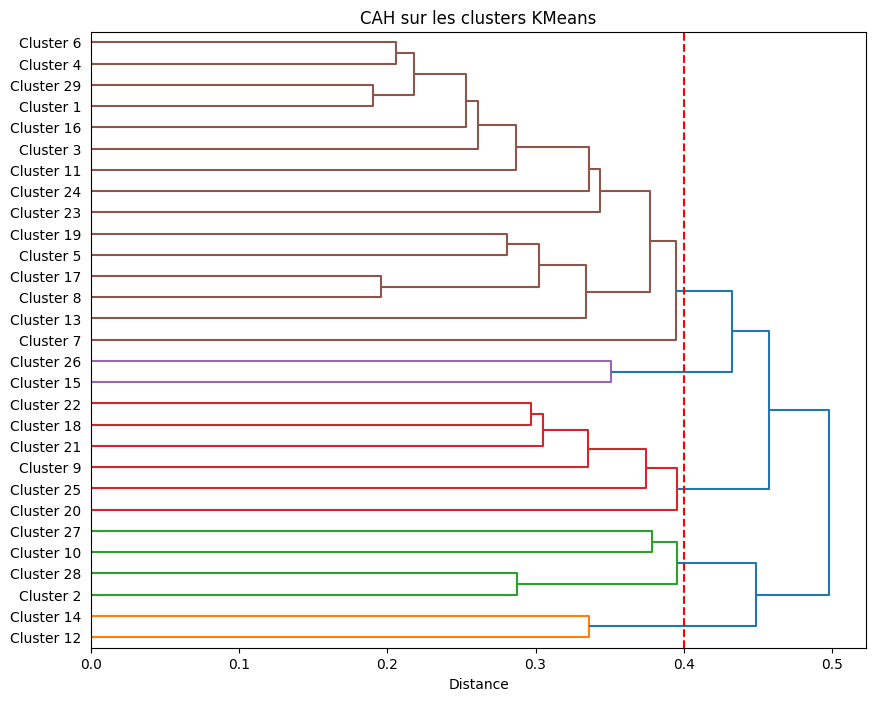
\includegraphics[width=\textwidth]{figure/dendrogramme.png}
    \caption{Dendrogramme de la classification hiérarchique des clusters K-means}
    \label{fig:dendrogramme}
\end{figure}

Dans cette analyse, le seuil de distance a été fixé à 0,40 afin de découper l’arbre hiérarchique en grandes familles de motifs. Ce regroupement rend les résultats plus lisibles : les 29 clusters initiaux peuvent être interprétés non seulement individuellement, mais aussi comme des ensembles thématiques plus larges. Cette organisation facilite ensuite la comparaison entre les motifs dominants du corpus et leur répartition dans les romans de Zola.

\subsubsection{Création des grandes familles de motifs}

À partir du dendrogramme, les clusters ont été regroupés en cinq grandes familles de motifs. Cette opération permet de simplifier l'analyse et de faire apparaître les grandes zones thématiques du corpus.

\begin{lstlisting}[language=Python, caption={Création des groupes CAH à partir des clusters K-means}]
groupes_cah = fcluster(Z, t=0.40, criterion="distance")

df_groupes = pd.DataFrame({
    "cluster": range(1, kmeans.n_clusters + 1),
    "groupe_cah": groupes_cah
})

df_groupes["nom_cluster"] = df_groupes["cluster"].map(
    noms_clusters_kmeans
)
\end{lstlisting}

Les groupes obtenus ont ensuite été nommés manuellement, en fonction des clusters qu'ils rassemblent.

\begin{lstlisting}[language=Python, caption={Nomination des grandes familles de motifs}]
noms_groupes_cah = {
    1: "Religion locale et autorite clericale",
    2: "Guerre, insurrection et conflit politique",
    3: "Institutions, croyances et encadrement social",
    4: "Argent, dettes et circulation financiere",
    5: "Vie quotidienne, espaces sociaux et experiences individuelles"
}

df_groupes["nom_groupe_cah"] = df_groupes["groupe_cah"].map(
    noms_groupes_cah
)
\end{lstlisting}

Ces grandes familles permettent d'obtenir une lecture plus synthétique des résultats. La première famille regroupe les thèmes liés à la religion locale et à l'autorité cléricale. La deuxième rassemble les motifs de guerre, d'insurrection et de conflit politique. La troisième renvoie aux institutions, aux croyances et aux formes d'encadrement social. La quatrième concerne l'argent, les dettes et les circulations financières. Enfin, la cinquième regroupe les motifs les plus liés à la vie quotidienne, aux espaces sociaux et aux expériences individuelles.

Cette structuration est particulièrement utile pour l'analyse littéraire, car elle permet de passer d'une liste de clusters nombreux à une organisation thématique plus lisible. Elle montre aussi que les motifs extraits par K-means ne sont pas isolés, mais peuvent être regroupés en ensembles plus larges correspondant à des dimensions importantes de l'œuvre de Zola.

\subsubsection{Attribution des grandes familles aux segments}

Une fois les groupes hiérarchiques définis, chaque segment du corpus a reçu une étiquette correspondant à la grande famille de motifs associée à son cluster. Cette opération permet d'analyser non seulement les clusters détaillés, mais aussi les grandes catégories thématiques dans lesquelles ils s'inscrivent.

\begin{lstlisting}[language=Python, caption={Attribution des groupes CAH aux segments du corpus}]
cluster_vers_groupe = dict(
    zip(df_groupes["cluster"], df_groupes["groupe_cah"])
)

df["groupe_cah"] = df["cluster"].map(cluster_vers_groupe)
df["nom_groupe_cah"] = df["groupe_cah"].map(noms_groupes_cah)
\end{lstlisting}

Cette étape permet de relier chaque paquet de phrases à deux niveaux d'analyse. Le premier niveau est le cluster K-means, qui fournit une catégorie thématique fine. Le second niveau est le groupe CAH, qui fournit une catégorie plus générale. Cette double échelle d'interprétation est utile car elle permet d'adapter le niveau de détail selon les besoins de l'analyse : on peut étudier les motifs précis, ou bien observer les grandes tendances du corpus.

\subsubsection{Analyse de la répartition des clusters}

Après la nomination des clusters et des grandes familles, plusieurs visualisations ont été produites afin d'étudier leur répartition dans le corpus. La première consiste à compter le nombre de segments associés à chaque grande famille de motifs.

\begin{lstlisting}[language=Python, caption={Nombre de segments par grande famille de motifs}]
counts = df["nom_groupe_cah"].value_counts().sort_values()

plt.figure(figsize=(10, 6))
counts.plot(kind="barh")

plt.title("Nombre de segments par grande famille de motifs")
plt.xlabel("Nombre de segments")
plt.ylabel("Groupe CAH")
plt.show()
\end{lstlisting}

Cette visualisation permet d'identifier les grandes familles les plus représentées dans l'ensemble du corpus. Elle donne une lecture globale de l'organisation thématique des segments. Une famille très représentée indique qu'un ensemble de motifs revient fréquemment dans les romans, tandis qu'une famille moins présente peut correspondre à un thème plus spécifique, associé à certains romans ou à certaines situations narratives.

Une seconde visualisation a été produite à l'échelle des clusters détaillés.


Cette représentation permet de voir quels clusters sont les plus fréquents dans le corpus. Elle est plus précise que l'analyse par grandes familles, car elle distingue les motifs thématiques particuliers. Elle permet par exemple d'observer séparément les clusters associés à la mine, à la finance, à la religion, à la famille ou au monde domestique.

\subsubsection{Distribution des clusters par œuvre}

Afin d'observer la présence des clusters dans chaque roman, une table croisée a été construite entre les fichiers du corpus et les clusters thématiques. La normalisation par ligne permet d'obtenir, pour chaque œuvre, la proportion de segments associés à chaque cluster.



Cette analyse est importante, car elle permet de relier les clusters aux romans. Certains clusters peuvent être très transversaux et apparaître dans de nombreuses œuvres, tandis que d'autres peuvent être fortement associés à un roman précis. Par exemple, un cluster lié à la mine peut être particulièrement représenté dans \textit{Germinal}, tandis qu'un cluster lié à la finance peut être plus présent dans \textit{L'Argent}. De la même manière, les clusters associés au commerce peuvent être importants dans \textit{Au Bonheur des dames}, et ceux liés à la guerre dans \textit{La Débâcle}.

Une analyse similaire a été réalisée au niveau des grandes familles de motifs.



Cette seconde visualisation offre une lecture plus synthétique. Elle permet de comparer les romans selon les grandes familles de motifs qui les structurent. Cette approche est particulièrement utile pour repérer des oppositions ou des proximités entre les œuvres : certains romans peuvent être dominés par des motifs de vie quotidienne, tandis que d'autres accordent plus de place aux institutions, à la religion, à la guerre ou aux conflits sociaux.

\subsubsection{Projection UMAP des segments}

Une projection UMAP a enfin été utilisée pour représenter les segments dans un espace en deux dimensions. Cette méthode de réduction de dimensionnalité permet de visualiser la manière dont les segments se répartissent selon leur proximité lexicale. Les points sont colorés selon leur grande famille de motifs.

\begin{lstlisting}[language=Python, caption={Projection UMAP des segments par grande famille de motifs}]
reducer = umap.UMAP(n_components=2, random_state=42)
X_umap = reducer.fit_transform(X)

plt.figure(figsize=(10, 7))

plt.scatter(
    X_umap[:, 0],
    X_umap[:, 1],
    c=df["groupe_cah"],
    cmap="tab10",
    s=10,
    alpha=0.7
)

plt.title("Projection UMAP des segments par grande famille de motifs")
plt.xlabel("UMAP 1")
plt.ylabel("UMAP 2")
plt.colorbar(label="Groupe CAH")
plt.show()
\end{lstlisting}

Cette visualisation ne doit pas être interprétée comme une preuve définitive de séparation entre les groupes, mais comme un outil exploratoire. Elle permet d'observer si les segments associés à une même famille de motifs tendent à se rapprocher dans l'espace vectoriel. Si certaines zones apparaissent relativement regroupées, cela peut indiquer que les familles thématiques correspondent à des structures lexicales cohérentes. À l'inverse, des zones plus mélangées peuvent signaler des motifs plus transversaux ou des segments hybrides.

\section{Comparaison des deux méthodes}

\subsection{Différences entre NMF et K-means}

Contrairement à la NMF, qui attribue à chaque segment un poids pour chacun des topics, K-means attribue chaque segment à un seul cluster. Cette différence est importante : la NMF autorise une lecture plus graduelle des thèmes, tandis que K-means produit une classification plus nette. Un segment appartient à un cluster principal, même s'il peut contenir plusieurs motifs thématiques.

La NMF permet donc d'observer la présence simultanée de plusieurs thèmes dans un même segment, alors que K-means propose une lecture plus catégorielle du corpus. Les deux méthodes ne répondent donc pas exactement au même objectif : la première met en évidence des topics latents, tandis que la seconde regroupe les segments selon leur proximité lexicale.

\subsection{Convergences thématiques}

Les intitulés obtenus montrent que les clusters couvrent des dimensions proches de celles observées avec la NMF. On retrouve par exemple des ensembles liés au travail, à la mine, à la finance, à la religion, à la famille, au monde domestique, à la guerre ou encore aux espaces urbains. Cette convergence entre les deux méthodes est intéressante, car elle indique que certains thèmes apparaissent de manière stable dans le corpus, indépendamment de la méthode utilisée.

\begin{figure}[H]
    \centering
    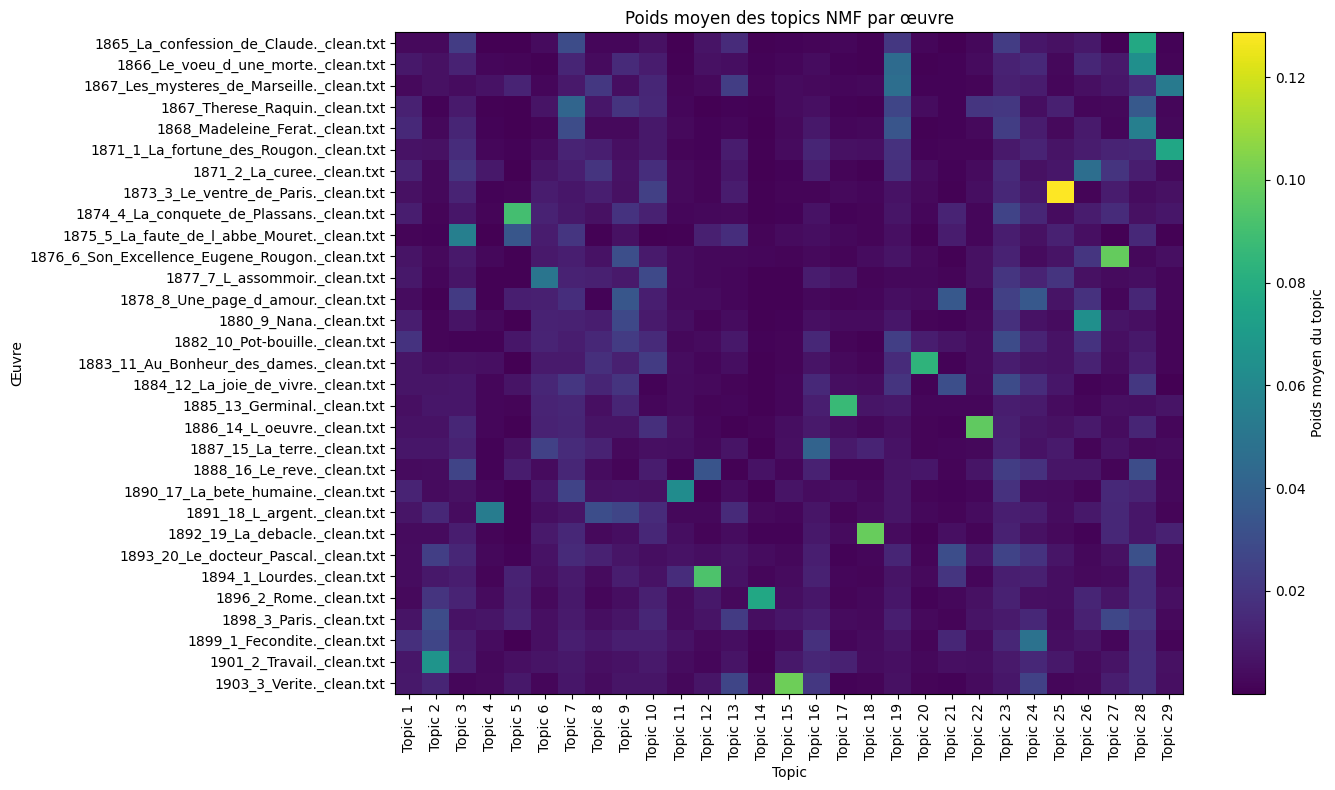
\includegraphics[width=\textwidth]{figure/headmap_nmf.png}
    \caption{Heatmap des poids des mots dans les topics NMF}
    \label{fig:heatmap_nmf}
\end{figure}
    
\begin{figure}[H]
    \centering
    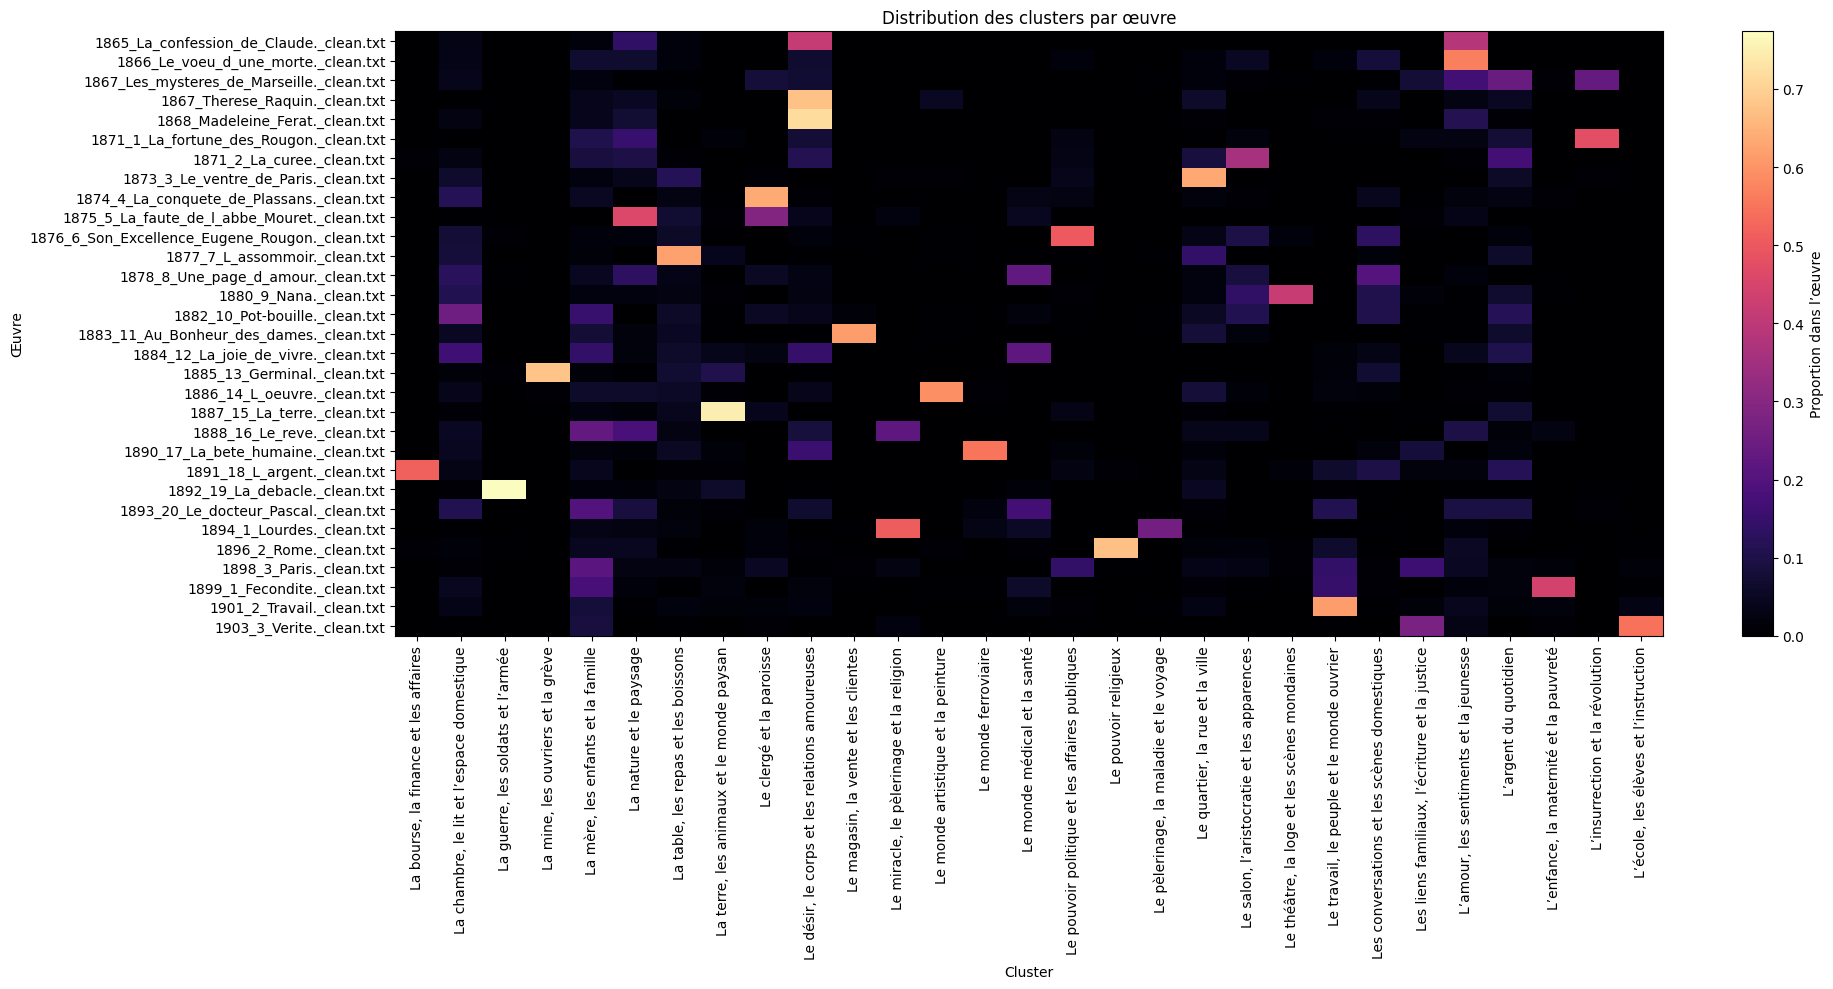
\includegraphics[width=\textwidth]{figure/headmap_kmeans.png}
    \caption{Heatmap des poids des mots dans les clusters K-means}
    \label{fig:heatmap_kmeans}
\end{figure}

La méthode K-means permet ainsi de compléter l'analyse réalisée avec la NMF. Elle offre une autre manière d'observer les régularités thématiques du corpus, non plus sous la forme de topics latents, mais sous la forme de groupes de segments lexicalement proches. Cette approche confirme plusieurs motifs déjà observés avec la NMF, notamment autour du travail, de la religion, de la famille, de l'argent, de la guerre, de la mine, du commerce ou de l'espace domestique.

\subsection{Distribution des thèmes par œuvre}

Afin d'observer la présence des clusters dans chaque roman, une table croisée a été construite entre les fichiers du corpus et les clusters thématiques. La normalisation par ligne permet d'obtenir, pour chaque œuvre, la proportion de segments associés à chaque cluster.

Cette analyse est importante, car elle permet de relier les clusters aux romans. Certains clusters peuvent être très transversaux et apparaître dans de nombreuses œuvres, tandis que d'autres peuvent être fortement associés à un roman précis. Par exemple, un cluster lié à la mine peut être particulièrement représenté dans \textit{Germinal}, tandis qu'un cluster lié à la finance peut être plus présent dans \textit{L'Argent}. De la même manière, les clusters associés au commerce peuvent être importants dans \textit{Au Bonheur des dames}, et ceux liés à la guerre dans \textit{La Débâcle}.

Une analyse similaire a été réalisée au niveau des grandes familles de motifs. Cette seconde visualisation offre une lecture plus synthétique. Elle permet de comparer les romans selon les grandes familles de motifs qui les structurent. Cette approche est particulièrement utile pour repérer des oppositions ou des proximités entre les œuvres : certains romans peuvent être dominés par des motifs de vie quotidienne, tandis que d'autres accordent plus de place aux institutions, à la religion, à la guerre ou aux conflits sociaux.

\subsection{Apport de la double approche}

Ainsi, K-means ne remplace pas la NMF, mais il constitue un complément méthodologique utile. En croisant les résultats des deux méthodes, il devient possible de distinguer les thèmes particulièrement stables de ceux qui dépendent davantage du modèle utilisé. Cette double approche renforce donc la solidité de l'analyse, tout en conservant une part d'interprétation qualitative indispensable dans l'étude d'un corpus littéraire.
\input{section/7_conclusion}
\newpage
\appendix
% Fichier annexe contenant les blocs de code de l'analyse.
% Ce fichier peut être inclus dans l'article principal avec :
% \input{article_zola_code}

\section{Annexe technique : code de l'analyse}

Cette annexe regroupe les principaux blocs de code utilisés pour préparer le corpus, lemmatiser les textes et appliquer les méthodes de modélisation thématique. Elle permet de conserver le corps de l'article principal plus lisible.

\subsection{Segmentation du corpus}

\begin{lstlisting}[language=Python, caption={Code de segmentation du texte en paquets de phrases}]
def segmenter_en_paquets(texte, taille_paquet=40):
    # Segmente le texte en paquets de phrases
    phrases = texte.splitlines()
    phrases = [p.strip() for p in phrases if p.strip()]
    paquets = []

    for i in range(0, len(phrases), taille_paquet):
        paquet = " ".join(phrases[i:i+taille_paquet])
        paquets.append(paquet)
    return paquets

rows = []

for _, row in df.iterrows():
    # Iteration sur chaque ligne du DataFrame
    paquets = segmenter_en_paquets(row["texte_brut"])

    for idx, paquet in enumerate(paquets):
        rows.append({
            "nom_fichier": row["nom_fichier"],
            "id_paquet": idx,
            "phrases_paquet": paquet
        })

df_phrases = pd.DataFrame(rows)
\end{lstlisting}

\subsection{Lemmatisation et filtrage lexical}

\begin{lstlisting}[language=Python, caption={Importation du modèle français de spaCy}]
nlp = spacy.load("fr_core_news_lg", disable=["ner", "parser"])
# Chargement du modele de langue francaise de spaCy.
# Les composants de reconnaissance des entites nommees et d'analyse
# syntaxique sont desactives afin d'accelerer le traitement.

nlp.max_length = 2_000_000
# Augmentation de la longueur maximale des textes traites par spaCy.
# Cette valeur est ajustable selon la taille des textes et la memoire
# disponible sur la machine.
\end{lstlisting}
\newpage
\begin{lstlisting}[language=Python, caption={Liste de stop words personnalisée}]
stop_word = {
    "je", "tu", "il", "elle", "ils", "elles", "nous", "vous",
    "me", "te", "se", "moi", "toi", "eux", "leur", "leurs",
    "ses", "mon", "ton", "son", "notre", "votre", "cette",
    "\u00e7a", "si", "m\u00eame", "o\u00f9", "dont", "sans",
    "quand", "bien", "l\u00e0", "sous", "\u00eatre", "avoir",
    "faire", "dire", "aller", "voir", "pouvoir", "demander",
    "prendre", "mettre", "parler", "devoir", "trouver", "donner",
    "comprendre", "savoir", "vouloir", "venir", "est", "ai",
    "as", "avez", "ont", "avaient", "\u00e9taient", "deux",
    "cent", "cents", "cinq", "dix", "vingt", "mille",
    "mme", "madame", "monsieur", "m", "mr", "mlle",
    "nana", "gervaise", "louis", "lazare", "etienne", "claude",
    "suzanne", "mouret", "rougon", "macquart", "saccard",
    "lacroix", "renn\u00e9e", "silv\u00e8re", "revert\u00e9gat",
    "mahoudeau", "ren\u00e9e", "xiii", "silv\u00e8re", "miette",
    "boccanera", "deberl", "daigremont", "lorilleu", "maheude",
    "cas", "f\u00e9licit\u00e9", "coupeau", "granou", "granoux",
    "gagni\u00e8re", "gagniere"
}
\end{lstlisting}
    

\begin{lstlisting}[language=Python, caption={Fonction de lemmatisation avec exclusion de mots spécifiques}]

def nettoyer_texte(texte):
    doc = nlp(texte)
    tokens = []

    for token in doc:
        lemme = token.lemma_.lower()

        if (
            not token.is_stop
            and not token.is_punct
            and not token.like_num
            and not token.is_space
            and token.pos_ in {"NOUN", "ADJ"}
            and len(lemme) > 2
            and lemme not in stop_word
        ):
            tokens.append(lemme)

    return " ".join(tokens)
\end{lstlisting}

\subsection{Vectorisation TF-IDF}
Le vectoriseur utilisé est défini de la manière suivante :

\begin{lstlisting}[language=Python, caption={Création de la matrice terme-document avec TF-IDF}]
vectorizer = TfidfVectorizer(
    min_df=3,
    max_df=0.8
)
X = vectorizer.fit_transform(df["phrases_lemm"])
\end{lstlisting}

\subsection{Modélisation par NMF}

% Coller ici les blocs lstlisting liés à l'entraînement et à l'interprétation de la NMF.

\subsection{Clustering par K-means}

% Coller ici les blocs lstlisting liés au clustering K-means et à la CAH.

\subsection{Visualisations}

% Coller ici les blocs lstlisting liés aux graphiques, distributions et projections UMAP.

\end{document}